In questo paragrafo viene introdotto con più dettagli il metodo proposto.
\section{Architettura del modello}
È stata creata un'architettura Deep Neural Network (DNN) basata su Gated Recurrent Unit (GRU) e Temporal Convolutional Neural Network (TCN) entrambe adattate al problema della classificazione multi-label. Il primo modello proposto, visibile in \ref{Figura 1.}, presenta una GRU con H unità nascoste (il numero H di unità nascoste è impostato a 50 nel nostro caso), seguito da un livello di max-pooling, da uno fully-connected e da un livello di output  sigmoid. L'approccio proposto per la TCN è il medesimo, con la differenza che il livello di max-pooling viene posto dopo il fully-connected.
\vspace{0.25cm} 
\begin{center}
	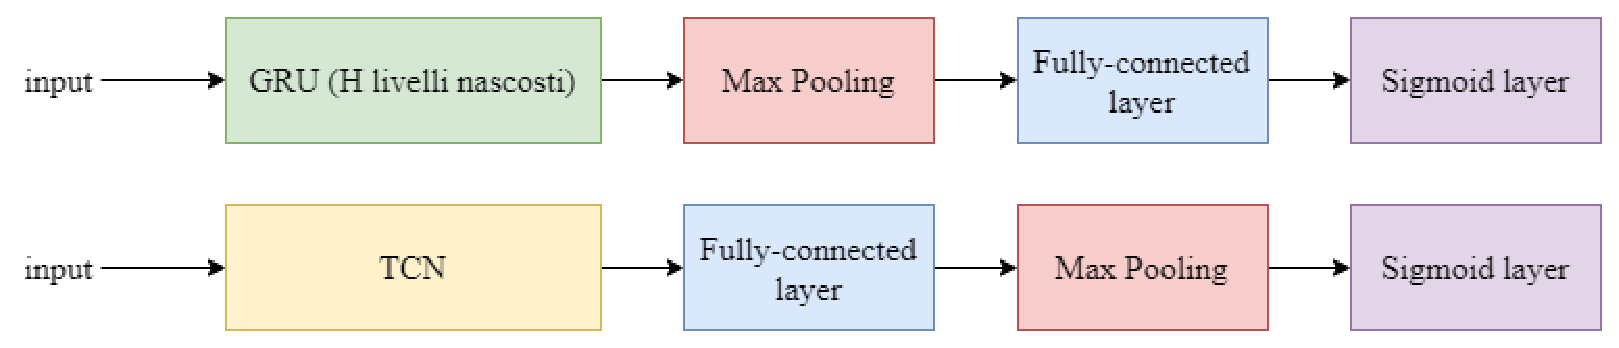
\includegraphics[scale=0.55]{images/arch.eps} %correggere GRU(H UNITA' nascoste)
	\captionof{figure}{Schema della DNN ricorrente}
	\label{appr:dnn}
\end{center}
\vspace{0.25cm}
Come \textit{loss function} è stata utilizzata la Binary Cross-Entropy calcolata dalle etichette predette e dalle etichette "obiettivo" (target-labels). La Binary Cross-Entropy calcola la perdita di una insieme di $ m $ osservazioni calcolando la seguente media:
\begin{equation}
	CELoss = -\frac{1}{m}\sum_{i=1}^{m}\sum_{j=1}^{l}y_{i}(j)\cdot\log(h_{i}(j))+(1-y_{i}(j))\cdot\log(1-h_{i}(j)) 
\end{equation}
dove $y_{i} \in \{0,1\}^l$ sono le etichette associate ad una istanza e $h_{i} \in \{0,1\}^l$  è il vettore delle etichette predette rispettivamente a ciascuna istanza.

\section{Pre-Processing}
Sebbene in molti problemi non si richiede un pre-processing dei dati d'input, ovvero una loro pre-elaborazione, prima di essere classificati tramite reti GRU, molto spesso invece questa è necessaria nel momento in cui tali dati sono feature vector che assumono valori con alta varianza. 

Il dataset di riferimento per questo elaborato è il dataset \textit{Liu}, che costituisce un collezione di farmaci raccolti per prevedere in silico i loro effetti collaterali. Una particolarità di questo dataset è il fatto che è estremamente sparso e ciò lo si può notare dal numero di features utilizzate per rappresentare ciascun pattern e il numero di etichette possibili. Un dataset che ha una tale peculiarità può rappresentare un problema soprattutto per la presenza dell'\textit{over-fitting}, ovvero una situazione in cui, a causa degli elevati gradi di libertà, il classificatore raggiunge un'elevata accuratezza sul Training-set, ma non sul Test-set e ciò lo porta ad "imparare a memoria" e a non generalizzare la predizione nel mondo reale.

Per evitare tale problematica è stata eseguita una riduzione di dimensionalità utilizzando diverse feature transform come PCA (Principal Component Analysis), t-SNE (t-Distributed Stochastic Neighbor Embedding) e KPCA (Kernel Principal Component Analysis).

\section{PCA}
forse spiego

\section{t-SNE}
forse spiego

\section{KPCA}
forse spiego

\section{Gated Recurrent Unit}
Gated Recurrent Unit (GRU) rappresenta una delle diverse tipologie di cella presente nelle reti neurali ricorrenti, introdotte nel 2014 da Kyunghyun Cho et al. (cita). GRU mira a risolvere principalmente il problema del vanishing (o exploding) gradient ovvero la scomparsa del gradiente. 

Tale problematica di sviluppa su reti neurali profonde e ne crea una difficoltà nell'addestramento tramite retro-propagazione dell'errore (backpropagation). Una delle principali cause è l'utilizzo di funzioni di attivazione non lineari standard, come la sigmoide, la tangente iperbolica o la funzione logistica, che sono caratterizzate dall'avere il gradiente a valori nell'intervallo $[0,1]$; ciò porta, nell'applicazione della regola di derivazione a catena, a far decrescere esponenzialmente i valori dei parametri del modello nei livelli lontani dall'output. Si dice che tali funzioni hanno un comportamento di tipo saturante.

La cella GRU può essere considerata come una variante semplificata della cella LSTM (Long-Short Term Memory) che cerca di mantenerne i vantaggi, riducendo parametri e complessità. Rispetto alla LSTM, GRU presenta un forget gate che permette alla rete di decidere quale parte della vecchia informazione è rilevante per comprenderne la nuova.

% prestazioni
GRU fornisce prestazioni simili a LSTM in problemi come lo speech signal modeling, polyphonic music modeling e natural language processing (citazione 11-12). Secondo (citazione 13-14) le celle GRU hanno prestazioni migliori su dataset di piccole dimensioni.

\vspace{0.25cm} 
\begin{center}
	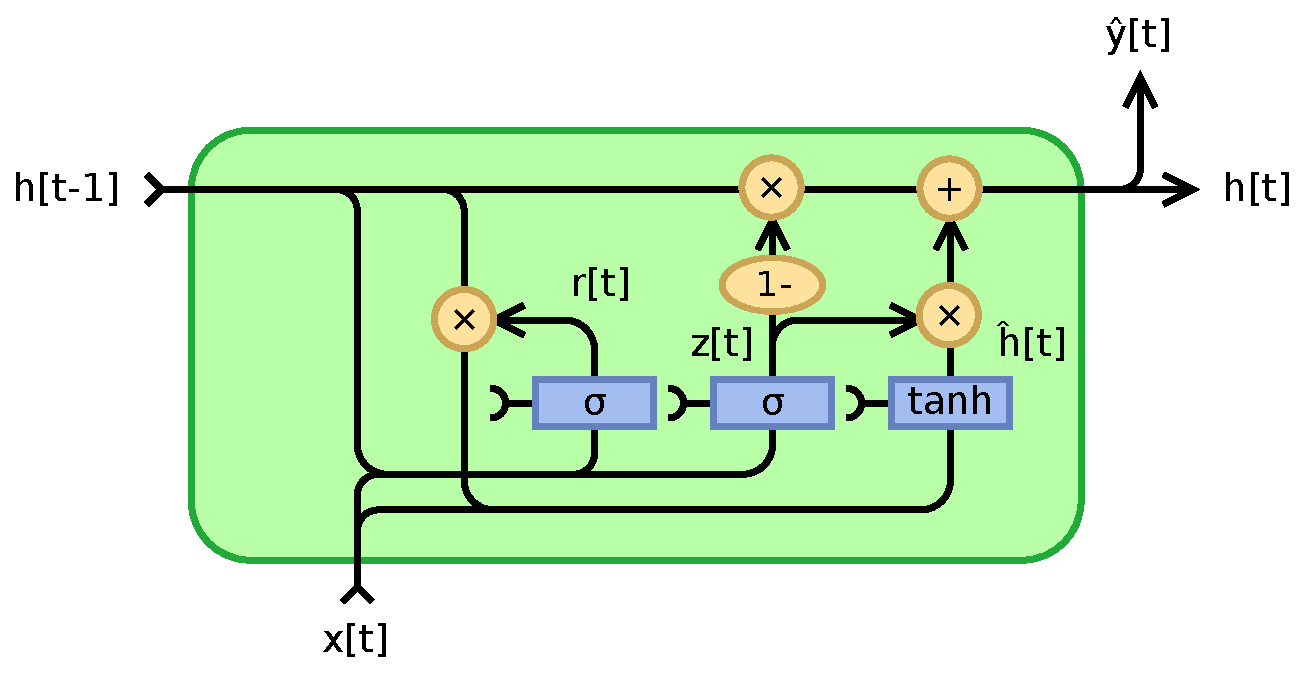
\includegraphics[scale=0.4]{images/gru2.eps}
	\captionof{figure}{Struttura di una cella GRU}
	\label{Figura 1.}
\end{center}
\vspace{0.25cm}

%componenti gru
Le componenti fondamentali di una cella GRU sono il reset gate e l'update gate: il primo determina quanta della passata informazione dimenticare mentre il secondo quale informazione può essere dimenticata e quale passata all'output. 

Sia $x_{t}$ la sequenza di input e $h_{t}$ quella di output; inizializziamo $h_{0}=0$ come lo stato di memoria della cella nell'istante $t=0$. Definiamo l'update gate vector $z_{t}$ e il reset gate vector $r_{t}$ come
\begin{equation}
	z_{t} = \sigma(W_{z}x_{t}+U_{z}h_{t-1}+b_{z}) 
\end{equation}
\begin{equation}
	r_{t} = \sigma(W_{r}x_{t}+U_{r}h_{t-1}+b_{r})
\end{equation}
dove $W_{z}$, $U_{z}$, $b_{z}$, $W_{r}$,$U_{r}$, $b_{r}$ sono parametri matrici e vettori e $\sigma$ è la funzione sigmoidea. 

Definiamo
\begin{equation}
	\hat{h_{t}} = \phi(W_{h}x_{t}+U_{h}(r_{t} \bigodot h_{t-1})+b_{h})
\end{equation}
come l'activation vector candidato, dove $\phi$ è la funzione di attivazione tangente iperbolica e $\bigodot$ è l'Hadamard product (o component-wise product).
Sapendo che il parametro $r_{t}$ determina la quantità di informazione passata che è rilevante per l'activation vector candidato, si ha che
\begin{equation}
	h_{t} = (1-z_{t}) \bigodot h_{t-1}+z_{t} \bigodot \hat{h_{t}} 
\end{equation}
è l'output vector, che va a rappresentare lo stato di memoria della cella nell'istante $t$.

\section{Temporal Convolutional Neural Network}
Le Temporal Convolutional Neural Network (TCN) (citazione?) sono una classe di reti neurali che sfrutta una gerarchia di convoluzioni per estrarre informazioni da sequenze di input o da serie temporali.
Generalmente i problemi legati alle serie temporali sono risolti da architetture di reti neurali ricorrenti (RNN) che, come sappiamo, introducono un modo per poter conservare e memorizzare l'informazione, ma Bai et al. \textbf{(citazione)} dimostra come reti neurali convoluzionali (CNN) possono eguagliare o addirittura superare le prestazioni delle reti ricorrenti.

La caratteristica più rilevante delle TCN è che utilizzano dei livelli convolutivi 1D impilati l'uno sull'altro per creare una rete profonda, utili poter eseguire la convoluzione sulla dimensione temporale.

Oltretutto, ognuno di questi livelli possiede un fattore di dilatazione (dilation factor) che aumenta esponenzialmente man mano che la rete diventa profonda, consentendo ai primi livelli di cercare informazioni molto vicine tra loro temporalmente e ai livelli più profondi di individuare dipendenze a lungo termine, in base alla feature estratta dai livelli precedenti. Ciò consente alle reti TCN ti avere un \textit{reciptive field} molto ampio, superando di fatto uno dei limiti presenti nelle architetture RNN. 

La dimensione del \textit{reciptive field} può essere calcolata come segue:
\begin{equation}
	R = (f-1)(2^K-1)+1
\end{equation}
dove $f$ è la dimensione del filtro usato nelle convoluzioni e $K$ è il numero di livelli convoluzionali.

Il \textit{fattore di dilatazione} delle convoluzioni è $2^{(k-1)}$, dove $k$ è il numero di livelli convoluzionali.

\vspace{0.25cm} 
\begin{center}
	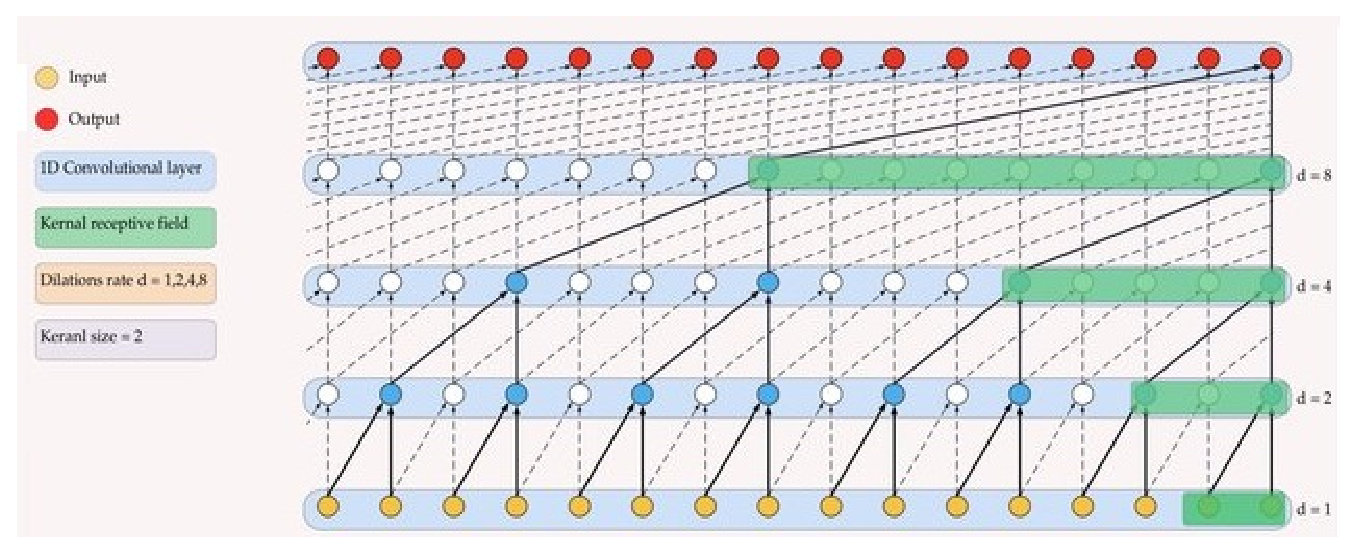
\includegraphics[scale=0.7]{images/esempio_tcn_dilatation.eps}
	\captionof{figure}{Esempio di struttura interna di una TCN, dove $d$ è il \textit{dilatation factor}}
	\label{Figura 1.}
\end{center}
\vspace{0.25cm}

% architettura tcn
L'architettura della TCN utilizzata nell'elaborato è formata da 4 blocchi, chiamati \textit{residual block}; ciascun blocco è costituito da due set ognuno dei quali comprende un livello convoluzionale dilatato casualmente, con 175 diversi filtri di dimensione $3x3$, seguito da un livello di attivazione ReLU, da un livello di Batch normalization e da un livello di Spatial dropout. L'input di ciascun blocco viene poi aggiunto all'output dello stesso (incluso un livello convoluzionale 1-by-1 opzionale, che si aggiunge quando il numero di canali tra l'input e l'output non coincidono).

Inoltre è stato utilizzato un livello fully-connected seguito da un livello di max-pooling ed, infine, come livello di output è stato utilizzato uno sigmoideo per ottenere la classificazione multiclasse.

Per l'addestramento è stato utilizzato un \textit{dropout factor} con probabilità 0.05.

\section{Pooling}
Dopo il nucleo principale della rete GRU/TCN è stato inserito un livello di Pooling, con lo scopo di ridurre la dimensionalità dei dati processati mantenendo solo l'informazione più rilevante e facendo diminuire la probabilità di overfitting, problema già accennato nell'introduzione. In particolare è stato utilizzato un livello di max-pooling lungo la dimensione temporale.

\section{Livello fully-connected e livello sigmoideo}
I livelli Fully-connected (o completamente connessi) in una rete neurale sono quei livelli in cui tutti gli input di un livello sono collegati a ogni unità di attivazione del livello successivo. Nei modelli di apprendimento  automatico più diffusi, gli ultimi livelli sono tipicamente completamente connessi, che hanno lo scopo di compialre i dati estratti dai livelli precedenti per formare l'output finale della rete. È il secondo livello più dispendioso in termini di tempo, dopo il livello Convoluzionale.
Il livello Fully-connected è composto da $l$ neuroni ($l$ è il numero di etichette di output di un dato problema) completamente connessi con i livelli precedenti. È stata utilizzata una funzione sigmoidea come funzione di attivazione nel livello finale in modo da riportare un valore di attivazione nell'intervallo $[0...1]$, che può essere interpretato come valore finale di probabilità per ogni etichetta. 

Pertanto, l'output del modello è un vettore di classificazione multi-label: l'output di ciascun neurone del livello fully-connected fornisce una votazione (che varia da 0 a 1) per una singola etichetta.

\vspace{0.25cm} 
\begin{center}
	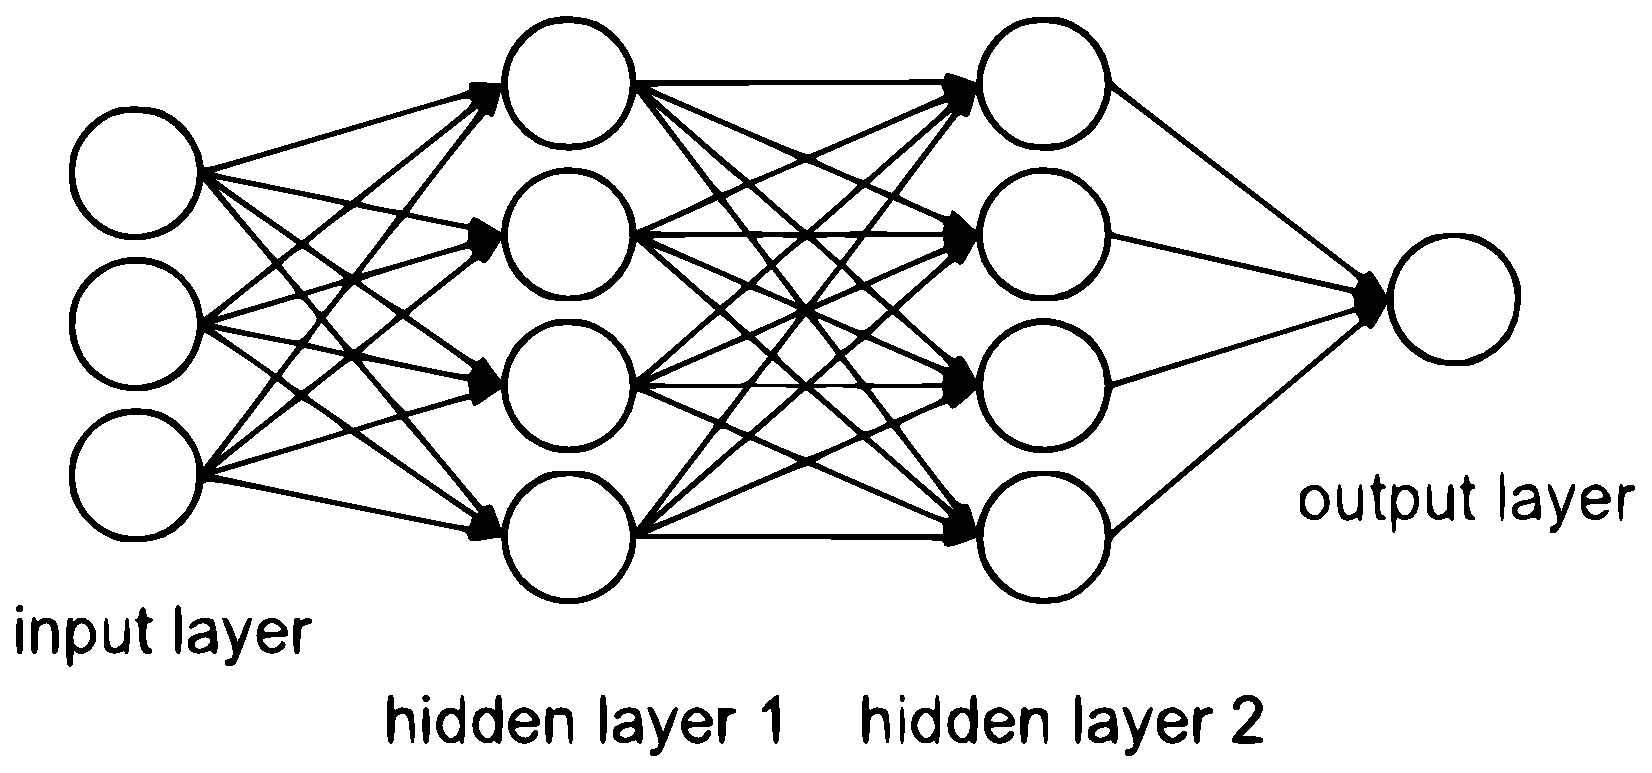
\includegraphics[scale=0.4]{images/neural_net2.eps}
	\captionof{figure}{Esempio di fully-connected layer}
	\label{Figura 1.}
\end{center}
\vspace{0.25cm}

\section{Addestramento}
L'addestramento viene eseguito utilizzando diverse varianti del metodo di ottimizzazione Adam che verranno presentate nel capitolo 5. È stato utilizzato un learning rate piuttosto alto pari a 0.01, un gradient decay di 0.5 e un squared gradient decay di 0.999.

Un altro passaggio effettuato è stato clippare il gradiente con una soglia pari a 1 utilizzando la L2-norm.

La dimensione di ciascun mini-batch è stata fissata a 30, mentre il numero di epoche è stato settato a 150 per GRU e 100 per TCN.

\section{Creazione degli ensemble}
Gli ensemble combinano l'output di più modelli per migliorare le prestazioni del sistema e contrastare l'overfitting. Un buon metodo per migliorare le previsioni e la generalizzazione dell'ensemble è aumentare la diversità dei classificatori. L'architettura degli ensemble è basata sulla fusione con average rule di diversi modelli addestrati sullo stesso problema. 

Gli ottimizzatori giocano un ruolo fondamentale nella ricerca del minimo della loss function: diverse strategie di ottimizzazione possono convergere a minimi locali diversi e quindi raggiungere diversi ottimi.

Sono stati valutati diversi ottimizzatori adatti alla creazione di ensemble: Adam Optimizer (cita), diffGrad (cita) e 4 nuove varianti di questo approccio, denominate DGrad, Cos1, Exp e Sto.

È stato costruito un ensemble di 40 reti neurali nel seguente modo: per ogni layer di ogni rete, viene scelto casualmente che variante di ottimizzazione utilizzare per quel layer. In questo modo si ottengono 40 differenti GRU e TCN.
